\documentclass[runningheads,envcountsect,envcountsame]{llncs}
\usepackage[utf8]{inputenc}
\usepackage[T1]{fontenc}
\usepackage{amsmath}
\usepackage{amssymb}
\usepackage{tikz}
\usetikzlibrary{arrows.meta}

\begin{document}

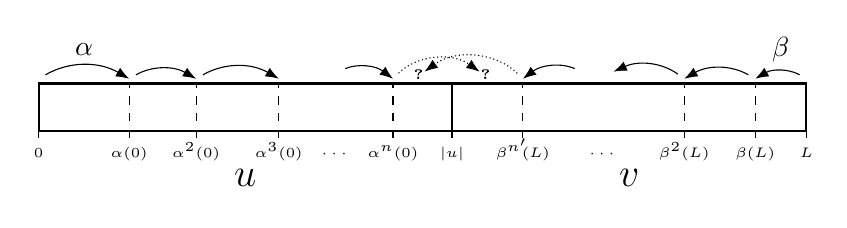
\begin{tikzpicture}[auto,x=5mm,y=3mm,anchor=mid,baseline,node distance=1.3em]

\def\xLz{0}
\def\xLu{10.5}
\def\xLuv{19.5}

\def\xuo{2.3};
\def\xui{4.0};
\def\xuii{6.1};
\def\xumi{\xLu-1.5};

\def\xvmo{\xLuv-1.3}
\def\xvmi{\xLuv-3.1}
\def\xvmii{\xLuv-4.9}
\def\xvi{\xLu+1.8}

{\tikzstyle{every node}=[node font=\Large]
 \node at ({(\xLz+\xLu)/2},-3) {$u$};
 \node at ({(\xLu+\xLuv)/2},-3) {$v$};
}

{\tikzstyle{every path}=[draw,thick,-]
\path (\xLz,-1.0) -- (\xLu,-1.0) -- (\xLu,1.0) -- (\xLz,1.0) -- cycle;
\path (\xLu,-1.0) -- (\xLuv,-1.0) -- (\xLuv,1.0) -- (\xLu,1.0) -- cycle;
}
{\tikzstyle{every path}=[draw,dashed,-]
\path (\xLz,-1.3)   -- (\xLz,1);
\path (\xLu,-1.3)   -- (\xLu,1);
\path (\xLuv,-1.3)   -- (\xLuv,1);
\path (\xuo,-1.3)   -- (\xuo,1);
\path (\xui,-1.3)   -- (\xui,1);
\path (\xuii,-1.3)   -- (\xuii,1);
\path (\xumi,-1.3)   -- (\xumi,1);
\path (\xvmo,-1.3)   -- (\xvmo,1);
\path (\xvmi,-1.3)   -- (\xvmi,1);
\path (\xvi,-1.3)   -- (\xvi,1);
}
{\tikzstyle{every node}=[node font=\tiny]
\node at (\xLz,-2) {$0$};
\node at (\xLu,-2) {$|u|$};
\node at (\xLuv,-2) {$L$};
\node at (\xuo,-2) {$\alpha(0)$};
\node at (\xui,-2) {$\alpha^2(0)$};
\node at (\xuii,-2) {$\alpha^3(0)$};
\node at (\xumi,-2) {$\alpha^n(0)$};
\node at ({(\xuii+\xumi)/2},-2) {$\cdots$};
\node at (\xvmo,-2) {$\beta(L)$};
\node at (\xvmi,-2) {$\beta^2(L)$};
\node at (\xvi,-2) {$\beta^{n'}\!\!(L)$};
\node at ({(\xvi+\xvmi)/2},-2) {$\cdots$};
}

{\tikzstyle{every path}=[-Latex,shorten <=1mm]
\path (\xLz,1.2) edge [bend left=30] node [above] {$\alpha$} (\xuo,1.2);
\path (\xuo,1.2) edge [bend left=30] (\xui,1.2);
\path (\xui,1.2) edge [bend left=30] (\xuii,1.2);
\path (\xuii + 1.5,1.5) edge [bend left=30] (\xumi,1.2);
\path (\xLuv,1.2) edge [bend right=30] node [above] {$\beta$} (\xvmo,1.2);
\path (\xvmo,1.2) edge [bend right=30] (\xvmi,1.2);
\path (\xvmi,1.2) edge [bend right=30] (\xvmii,1.5);
\path (\xvi + 1.5,1.5) edge [bend right=30] (\xvi,1.2);
}
{\tikzstyle{every path}=[-Latex,shorten <=1mm,dash pattern=on \pgflinewidth off 1pt,bend left=40]
 \node[minimum size=0pt,font=\tiny] (tip1) at (\xLu + 0.85, 1.4){\textbf{?}};
 \node[minimum size=0pt,font=\tiny] (tip2) at (\xLu - 0.85, 1.4){\textbf{?}};
 \path (\xumi,1.2) edge [bend left=40] (\xLu + 0.7, 1.5);
 \path (\xvi,1.2) edge [bend right=40] (\xLu - 0.7, 1.5);
}


\end{tikzpicture}

\end{document}